\documentclass[8pt]{article}
\usepackage{latexsym}
\usepackage[UTF8]{ctex}
\usepackage{geometry}
\geometry{a4paper,left=2.5cm,right=2.5cm,top=2cm,bottom=2cm}
\usepackage{amsmath}  
\usepackage{amssymb}  
\usepackage{CJK}
\usepackage{enumitem}
\usepackage{graphicx}
\usepackage{titletoc}

\begin{document}
\let\nofiles\relax

\zihao{4}

\titlecontents{section}[10mm]
{\fontsize{10pt}{14pt}\selectfont \CJKfamily{hei}}
{\contentslabel{4em}}
{}
{\titlerule*{.}\contentspage}
\titlecontents{subsection}[12mm]
{\fontsize{10pt}{14pt}\selectfont \CJKfamily{song}}
{\contentslabel{2em}}
{}
{\titlerule*{.}\contentspage}
\titlecontents{subsubsection}[23mm]
{\fontsize{10pt}{14pt}\selectfont \CJKfamily{song}}
{\contentslabel{3em}}
{}
{\titlerule*{.}\contentspage}

\title{生物智能算法课程报告-粒子群算法}
\author{王梁\quad21621254}
\date{}
\maketitle
\tableofcontents

\newpage
\section{粒子群算法简介}
\vspace{0.1cm}
\subsection{PSO的提出}
粒子群算法,也称作粒子群优化算法(Particle Swarm Optimization, 缩写为PSO),是群体智能算法的一种。1995年由Eberhart和Kennedy源于对鸟群捕食行为的研究提出PSO算法。该算法受到飞鸟集群活动的规律性启发,利用群体中的个体对信息的共享,按照一定的规则调整单个个体的运动,从而使整个群体的运动在问题求解空间中产生从无序到有序的演化过程,从而获得最优解。
\subsection{生态学场景}
粒子群算法尝试模拟如下场景:
一群鸟随机的分布在一个区域中,在这个区域里只有一块食物。所有的鸟都不知道食物在哪里,但是它们知道当前的位置离食物有多远。那么对于每一只鸟而言,找到食物的最优策略是什么呢?最简单有效的方法就是追寻自己视野内目前离食物最近的鸟。
如果把食物当做一个优化问题的最优点,而把鸟离食物的距离当做函数的话,那么鸟群觅食的过程就可以当做一个函数寻优的过程。受此启发经过抽象和简化提出了粒子群算法。
\subsection{基本思想}
每个优化问题的潜在解都是搜索空间中的一只鸟,称之为“粒子”。所有的粒子都有一个被优化的函数决定的适应值(fitness value),每个粒子还有一个矢量速度决定他们飞翔的方向和距离。然后粒子就追随当前的最优粒子在解空间中搜索,通过迭代找到最优解。\par
PSO算法初始化为一群随机粒子(随机解)。在每一次迭代中,粒子通过跟踪两个“极值”来更新自己: 一是粒子本身在过去所找到的最优解;二是整个种群目前找到的最优解,这两个值分别对应种群中的个体认知和群体认知。粒子的速度根据这两个值进行调整。最终当被优化函数的值低于设定值或者迭代次数高于设定值时,迭代过程停止。

\section{标准PSO算法}
\subsection{PSO算法要素}
\begin{itemize}[leftmargin=2em]
	\setlength{\itemsep}{0pt}
	\setlength{\parsep}{0pt}
	\setlength{\parskip}{0pt}
	\item D维空间: 优化问题的解空间。
	\item 粒子: 解空间中的一个随机解,其位置和速度都是D维。
	\item 适应度函数: 优化问题, 代入粒子当前位置可得一个函数值。
	\item 个体最佳位置: 粒子i经历过的最好位置 $pbest_i = (p_{i1}, p_{i2}, ..., P_{iD})$
	\item 种群最佳位置: 整个种群经历过的最好位置 $gbest = (g_1, g_2, ..., g_D)$
\end{itemize}
\par
通常, 在第d维$(1<=d<=D)$的位置变化范围限定在$[X_{min,d},X_{max,d}]$内,速度变化范围限定在$[-V_{max,d},V_{max,d}]$内。

\subsection{迭代过程}
粒子i的速度更新公式:
\begin{equation}
	V_i = w * V_i + c_1 * r_1 * (pbest_i - X_i) + c_r * r_2 * (gbest_d - X_i)
\end{equation}
\par
粒子i的位置更新公式:
\begin{equation}
	X_i = X_i + V_i
\end{equation}
各变量的含义分别是:
\begin{itemize}[leftmargin=2em]
	\setlength{\itemsep}{0pt}
	\setlength{\parsep}{0pt}
	\setlength{\parskip}{0pt}
	\item $V_i$: 第i个粒子的速度
	\item $X_i$: 第i个粒子的位置
	\item $c_1, c_2$: 加速度常数,调节学习的最大步长
	\item $r_1, r_2$: 两个随机函数,取值范围[0,1], 以增加随机搜索性
	\item $w$:惯性权重, 非负数, 调节对解空间的搜索范围
\end{itemize}

\par
粒子速度的更新包含三个部分: 粒子先前的速度,即惯性部分;“认知”部分,表示粒子自身的经验;“社会”部分,表示粒子间的信息共享。粒子的速度由这三个量决定。

\centerline{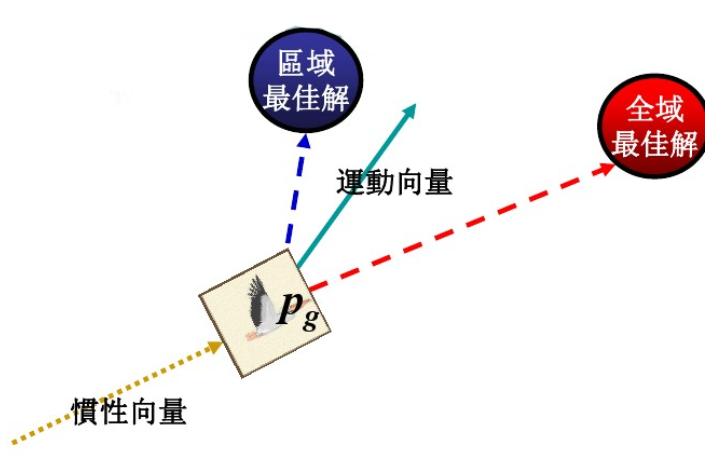
\includegraphics[width=0.5\textwidth]{1.png}}

\subsection{算法流程}
标准PSO算法的流程如下:
\begin{itemize}[leftmargin=4em]
	\setlength{\itemsep}{0pt}
	\setlength{\parsep}{0pt}
	\setlength{\parskip}{0pt}
	\item[1] 初始化粒子群体, 包括随机速度和位置。 群体规模为n
	\item[2] 根据适应度函数, 计算每个粒子的适应度函数值
    \item[3] 更新每个粒子的个体历史最佳位置
    \item[4] 更新种群的历史最佳位置
    \item[5] 更新每个粒子的速度和位置
	\item[6] 判断结束条件,否则返回步骤2

结束条件通常为最大迭代次数或者达到要求的最佳适应值
\end{itemize}

\subsection{参数调节}
在实际应用中,粒子群算法的参数设置对算法结果有较大的影响,但在不同的问题中,并没有一个完全清晰地调整参数的最优策略,往往依据经验尝试。各个参数对算法结果的影响如下:
\subsubsection{种群大小}
	种群大小n是一个整型参数。n很小,陷入局部最优的可能性很大,算法得不到最优解;n很大,算法的优化能力很好,但增加了计算时间。
	当群体数目增长至一定水平时,再增长将不会有显著的作用。
\par
	n一般取20-40, 对于大部分问题已经可以取得较好的结果。对于搜索空间较大或特定类别的问题,n可以取到100-200.

\subsubsection{惯性因子}
	惯性因子w使粒子下一次运动的速度受到当前速度的影响,从而使粒子不至受到周围最优点的影响而迅速转向,导致粒子的搜索空间变小,易陷入局部最优。w越小,粒子对自身速度的记忆越弱,收敛越快,但易陷入局部最优;w越大,粒子的搜索能力越强,不易陷入局部最优,但收敛速度变慢,收敛精度降低。
\par
	在实际中w不宜设定为一个常数,而是应该随着迭代次数变化。

\subsubsection{学习因子}
	学习因子$c_1, c_2$调节粒子受自身经验和群体信息影响的比例。若$c_1=0$,则成为“无私型粒子群算法”,粒子只受限于群体信息,而没有自身的记忆,算法会迅速丧尸群体多样性,容易陷入局部最优而无法逃脱。若$c_2=0$, 则成为“自我认知型粒子群算法”,粒子只受限于自身记忆,而不顾群体信息,算法的收敛速度会非常缓慢。一般情况下都会使$c_1,c_2$都不为0, 保持收敛速度和搜索效果的均衡。
\par
	$c_1,c_2$通常等于2。如果改变其取值,也通常在0-4之间。

\subsubsection{最大速度}
	粒子在更新速度时,其速度不能超过最大速度$V_m$。$V_m$较大时,算法搜索能力强,但粒子容易飞过最优解;$V_m$较小时, 不容易错过最优,但容易陷入最优。
\par	
	$V_m$一般设为每维变量变化范围的10\%-20\%。

\section{PSO算法的优缺点}
\subsection{优点}
粒子群算法的优点如下:
\begin{itemize}[leftmargin=4em]
	\setlength{\itemsep}{0pt}
	\setlength{\parsep}{0pt}
	\setlength{\parskip}{0pt}
	\item[1] PSO算法没有交叉和变异运算,依靠粒子的速度完成搜索,并且在迭代进化中只有最优的粒子把信息传递给其他粒子,搜索速度快。
	\item[2] 采用实数编码,易于描述和理解。
	\item[3] 只有非常少的参数需要调整。
	\item[4] 收敛速度较快。
	\item[5] 对优化问题定义的连续性无特殊要求。
	\item[6] 无集中控制约束,不会因为个体的故障而影响整个问题的求解,确保了系统具备很强的鲁棒性。这在一些实际的应用场景比较重要。
	\item[7] 相对于其它的演化算法,只需要较小的演化群体。
	\item[9] 易于并发
\end{itemize}

\subsection{缺点}
粒子群算法的缺点如下:
\begin{itemize}[leftmargin=4em]
	\setlength{\itemsep}{0pt}
	\setlength{\parsep}{0pt}
	\setlength{\parskip}{0pt}
	\item[1] PSO算法提供了全局搜索的可能,但是目前并不能严格证明其在全局最优点上的收敛性。由于PSO算法提出的时间不长,数学基础较为薄弱,在收敛性理论,计算性能,实现技术和参数的设置等方面缺乏严密的数学基础,其应用大多数仍然依靠经验和实验,理论研究大大滞后于PSO在工程中的应用。
	\item[2] 缺乏速度的动态调节,容易陷入局部最优而无法逃出。
	\item[3] 对于不同的问题,需要自己设计更新公式和有效的均衡全局搜索和局部改进的策略。
\end{itemize}

\section{PSO算法的改进}
\subsection{惯性权重衰减}
如前所述,惯性权重描述粒子上一代速度对当前速度的影响。w值较大,全局寻优能力强,局部寻优能力弱;反之,则局部寻优能力强。当问题解空间较大时,为了在搜索速度和搜索精度之间达到平衡,通常做法是采取类似模拟退火算法的思想,使算法在前期有较高的全局搜索能力以得到合适的种子,而在后期有较高的局部搜索能力以提高收敛精度。所以w不宜为一个固定常数。
\subsubsection{线性递减权值}
惯性权重w更新公式为:
\begin{equation}
	w = w_{max} - (w_{max} - w_{min}) * \frac{run}{run_{max}}
\end{equation}
\par
$w_{max}$是最大惯性权重,$w_{min}$是最小惯性权重,$run$是当前迭代次数,$run_{max}$是算法总迭代次数. 随着迭代次数的增加,惯性权重w不断减小,从而使PSO算法在初期具有较强的全局收敛能力,不易陷入局部最优无法逃脱,而后期具有较强的局部搜索能力,提高搜索精度,同时稳定落在最优解内。
\subsubsection{收缩因子法}
线性递减权值的方法不能避免后期因w过小而失去探索新区域的能力的问题。1999年,Clerc和Kennedy引入了收缩因子以保证算法的收敛性。该方法采用随机近似理论(stochastic approximation theory)分析PSO的动态行为,提取了一种使w随更新代数递减至0的取值策略。
速度更新公式为:
\begin{equation}
	V = K[V_i + c_1 * r_1 *(pbest_i - X_i) + c_2 * r_2 *(gbest - X_i)]
\end{equation}
其中,新增的收缩因子K收到学习因子$c_1,c_2$的限制,公式如下:
\begin{equation}
	K = \frac{2}{|2 - c - \sqrt{c^2 - 4c}|}, c = c_1 + c_2, c > 4
\end{equation}
通常取$c=4.1$, 从而$K=0.729, c1=c2=1.49445$.

\subsection{局部PSO和邻域拓扑}
根据粒子邻域是否为整个种群,PSO分为全局模型gbest和局部模型lbest. 对于gbest模型,每个粒子与整个群体的其它粒子进行信息交换,并向所有粒子中的历史最佳位置移动。gbest模型虽然具有较快的收敛速度,但是更容易陷入局部最优。为了克服gbest模型的缺点,lbest模型则限制每个粒子的只能获取其周围一个邻域内的其它粒子的信息。lbest模型能一定程度避免PSO算法陷入局部最优。

\subsubsection{空间邻域}
空间邻域是指直接在优化问题解空间按粒子间的距离(如欧式距离)进行划分。例如,Suganthan\cite{art1}提出,在搜索初始阶段,将邻域定义为每个粒子自身,随着迭代次数的增加,将邻域范围逐渐扩展到整个种群,汇总各个局部的最优值。具体而言,在迭代中计算每一个粒子与种群中其他粒子的距离,并记录任何两个粒子之间的最大距离为$dm$. 对每一个粒子按照$\frac{|X_a-X_b|}{dm}$计算一个比值,当该比值低于某一个阈值时则认为b在a的邻域中。其中$|X_a-X_b|$是粒子a到粒子b的距离,阈值的选择随着迭代次数变化。
\par
这种方法在实验中取得了较好的效果,但是由于需要计算所有粒子两两之间的距离,因而计算量较大,而且需要很大的存储空间,在实际中不经常使用。

\subsubsection{性能邻域}
性能邻域是根据性能指标(如适应度)划分的邻域。 例如,Kalyan\cite{art2}提出基于适应度距离比(fitness-distance-ratio, 缩写FDR)的邻域划分方案,两个粒子的距离采用如下度量:
\begin{equation}
	FDR(j, i, d) = \frac{Fitness(P_j) - Fitness(X_i)}{|P_{jd} - X_{id}|}
\end{equation}
其中,$p_j$是粒子j的历史最佳位置,$d$代表当前计算的是位置向量的第$d$维。当两个粒子j和i的FDR距离小于某一个阈值,则认为j在i的领域中。

\subsubsection{社会关系邻域}
社会关系邻域通常按照粒子的序列编号进行划分,这也是研究最多的一种划分方案。目前已有的拓扑方案有:环形拓扑, 轮形拓扑, 星型拓扑,塔形拓扑,冯诺依曼拓扑以及随机拓扑等。\\
\centerline{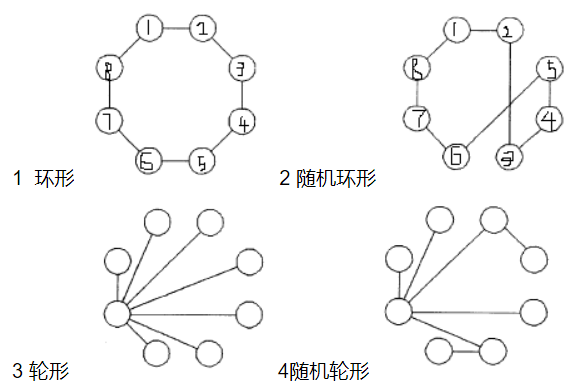
\includegraphics[width=0.5\textwidth]{2.png}}

\centerline{四种局部邻域拓扑方案}
针对不同的应用场景,这些拓扑的性能表现各异,但是一般而言,随机拓扑对大多数问题表现较好,其次是冯诺依曼拓扑。

\subsection{混合模型}
混合模型就是将其他进化算法或者传统优化算法应用到PSO中,用于提高粒子多样性,增强粒子的全局搜索能力或局部搜索能力,增强收敛速度与精度。结合的途径通常有两种:一是利用其它技术自适应调整收缩因子/惯性权重等,二是将PSO与其他进化算法操作算子结合。一下列举一些结合方法:
\begin{itemize}[leftmargin=2em]
	\setlength{\itemsep}{0pt}
	\setlength{\parsep}{0pt}
	\setlength{\parskip}{0pt}
	\item[1] 将PSO与蚁群算法结合,用于求解离散优化问题
	\item[2] 将种群动态地划分为多个子群,每个子群利用蚁群算法或者PSO进行独立优化
	\item[3] 将PSO与GA结合,用于天线优化设计和递归神经网络
	\item[4] 利用差分进化操作选择速度更新公式中粒子的最佳位置
	\item[5] 利用变异、选择和繁殖多种操作同时自适应确定速度更新公式中的邻域最佳位置以及惯性权重和加速度常数
\end{itemize}

\section{PSO算法的应用}
目前PSO算法的应用主要包含以下几个方面:
\begin{itemize}[leftmargin=2em]
	\setlength{\itemsep}{0pt}
	\setlength{\parsep}{0pt}
	\setlength{\parskip}{0pt}
	\item[1] 函数优化: 多极值函数求全局最优解,组合优化,约束优化,多目标优化,动态系统优化
	\item[2] 神经网络训练:将神经网络的所有参数(假设数目为D)看成一个D维空间的点,适应度函数则是神经网络的损失函数。相比常用的梯度下降,使用PSO算法优化神经网络参数收敛速度较快。
	\item[3] 工程应用: 电力系统,自动控制,机器人,任务分配,最优路径规划, 最优控制问题
	\item[4] 数据聚类: 聚类,模式识别与图像分类
\end{itemize}

% \renewcommand\refname{Reference}
\bibliographystyle{plain}
\bibliography{PSO}
\end{document}


